\documentclass{beamer}
% Importar a biblioteca para figuras
\usepackage{graphicx}
% Pacote hyperref
\usepackage{hyperref}
\usepackage[utf8]{inputenc}
\usepackage[T1]{fontenc}
\AtBeginDocument{\renewcommand{\figurename}{Figura}}
\AtBeginDocument{\renewcommand{\tablename}{Tabela}}
%\usepackage[brazil]{babel}
\usepackage{caption}
% Tema e cores
\usetheme{Singapore}
\usecolortheme{dove}
% Configuração do rodapé
\setbeamertemplate{footline}[frame number]


% Informações da apresentação
\title{2ª Mostra de PI da UNIVESP:}
\subtitle{Compartilhando Experiências e Dicas}
\author{Paulo Roberto Pereira Santiago}
\institute{Universidade Virtual do Estado de São Paulo\\ Polo Sertãozinho}
\date{\today}
\titlegraphic{
\includegraphics[width=3cm]{univesp.png}} % Ajuste a largura conforme necessário

\begin{document}

\begin{frame}
  \titlepage
\end{frame}

\begin{frame}
  \frametitle{Índice}
  \tableofcontents
\end{frame}

% Seção 1
\section{Resultado}

\begin{frame}
  \frametitle{Resultado do Projeto}
  \begin{block}{}
    - Relatório: PDF\\
    - Vídeo: YouTube\\
    - Exemplos: \href{https://apps.univesp.br/tcc-pi/pi/}{https://apps.univesp.br/tcc-pi/pi/}
  \end{block}
\end{frame}

\begin{frame}
  \frametitle{Resultado do Projeto}
  \begin{block}{}
    \begin{figure}
      \centering
      
\includegraphics[width=0.5\textwidth]{nota10.png} % Substitua com o caminho para sua imagem
      \captionsetup{labelformat=simple, labelsep=period}
      \caption{Só vou tirar 10!}
    \end{figure}
  \end{block}
\end{frame}

\begin{frame}
  \frametitle{Resultado do Projeto}
  \begin{block}{}
    \begin{center}
      É muito melhor que não fazer nada e desistir!
    \end{center}
    \begin{figure}
      \centering
      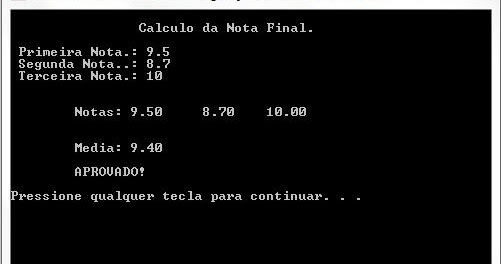
\includegraphics[width=0.5\textwidth]{nota9.jpg} % Substitua com o caminho para sua imagem
      \captionsetup{labelformat=simple, labelsep=period}
      \caption{Nota entre 8 - 9.5 está ótimo!}
    \end{figure}
  \end{block}
\end{frame}


% Seção 2
\section{Tema}
\begin{frame}
  \frametitle{Tema Escolhido}
  \begin{block}{}
    O Tema é da UNIVESP!
    \begin{figure}
      \centering
      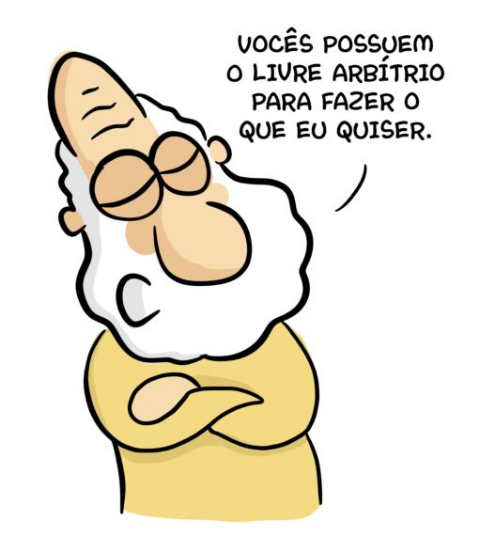
\includegraphics[width=0.4\textwidth]{univesp_tema_pi.png} % Substitua com o caminho para sua imagem
      \captionsetup{labelformat=simple, labelsep=period}
      \caption{A UNIVESP mostra o Norte!}
    \end{figure}
  \end{block}
\end{frame}

% Seção 3
\section{Escolha}
\begin{frame}
  \frametitle{Escolha do Tema}
  \begin{block}{\centering{Não se trata de um Prêmio Nobel, mas sim de um Projeto Integrador!}}
      \begin{figure}
      \centering
      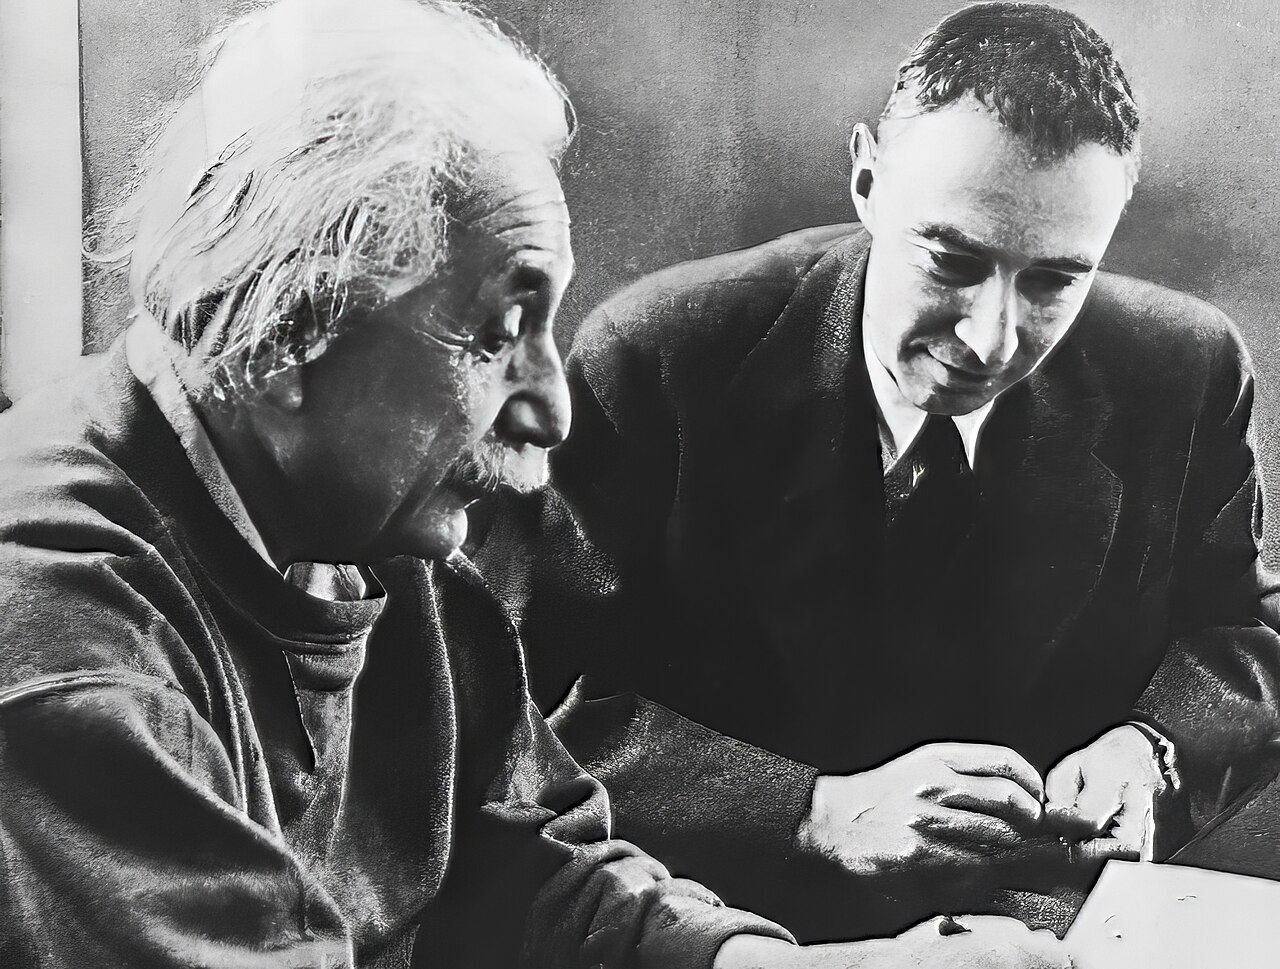
\includegraphics[width=0.4\textwidth]{Einstein_oppenheimer.jpg}
      \captionsetup{labelformat=simple, labelsep=period}
      \caption{Escute todos do grupo!}
    \end{figure}
    Execute a ideia mais viável e promissora do grupo o quanto antes. De preferência por algo que você consegueria fazer sozinho!
  \end{block}
\end{frame}

% Seção 4
\section{Equipe}
\begin{frame}
  \frametitle{Trabalho em Equipe}
  \begin{block}{Dinâmica de Equipe:}
        \begin{figure}
      \centering
      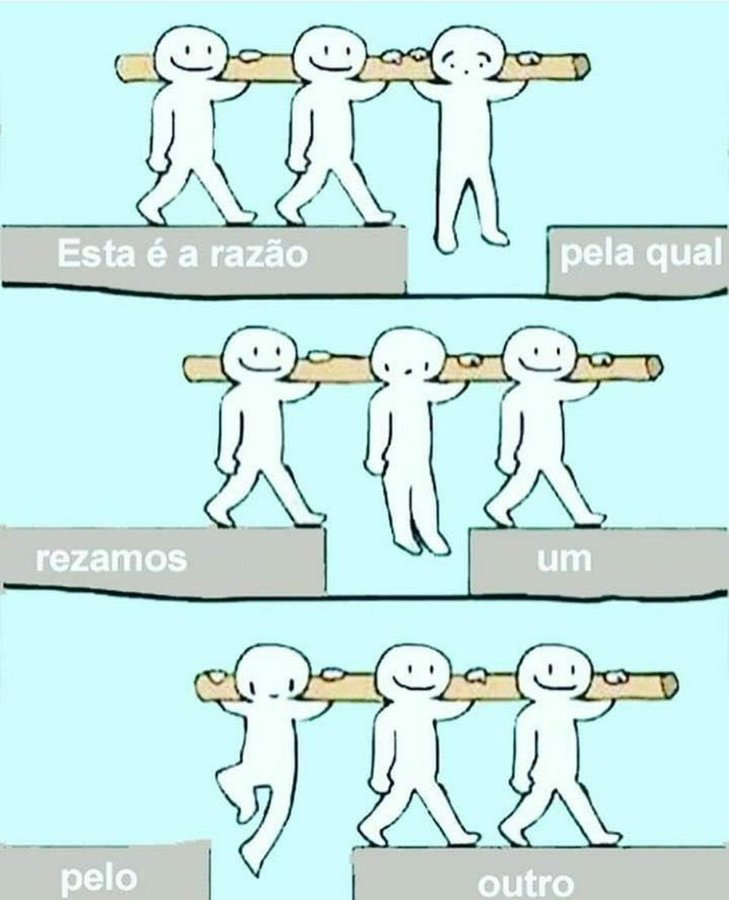
\includegraphics[width=0.4\textwidth]{juntos.jpg}
      \captionsetup{labelformat=simple, labelsep=period}
      \caption{Não precisa explicar né!}
    \end{figure}
  \end{block}
\end{frame}

% Seção 5
\section{Reuniões}
\begin{frame}
  \frametitle{Reuniões de Equipe}
  \begin{block}{}
    Presencial ou por vídeo até definir o projeto.\\
    Depois, comunicação via WhatsApp e outros meios.\\
    Fazer mais e conversar menos!
    \begin{figure}
      \centering
      
\includegraphics[width=0.3\textwidth]{reunioes.jpg} % Substitua com o caminho para sua imagem
      \captionsetup{labelformat=simple, labelsep=period}
      \caption{Afinal Alguém/Grupo vai ter que fazer!}
    \end{figure}
  \end{block}
\end{frame}

% Seção 6
\section{Orientador}
\begin{frame}
  \frametitle{Participação do Orientador}
  \begin{block}{Orientador: Não é membro do grupo!}
    % Como o orientador contribuiu
    \begin{figure}
      \centering
      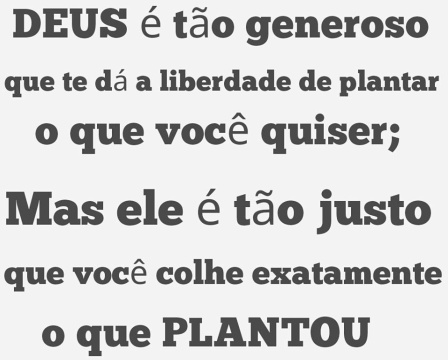
\includegraphics[width=0.5\textwidth]{arbitrio.jpg} % Substitua com o caminho para sua imagem
      \captionsetup{labelformat=simple, labelsep=period}
      \caption{Se vocês já sabem o que vão fazer e como fazer.\\
      Então, façam!}
    \end{figure}
  \end{block}
\end{frame}

% Seção 7
\section{Dicas}
\begin{frame}
  \frametitle{Outras Dicas - "Mão na Roda"}
  \begin{block}{}
    \begin{figure}
      \centering
      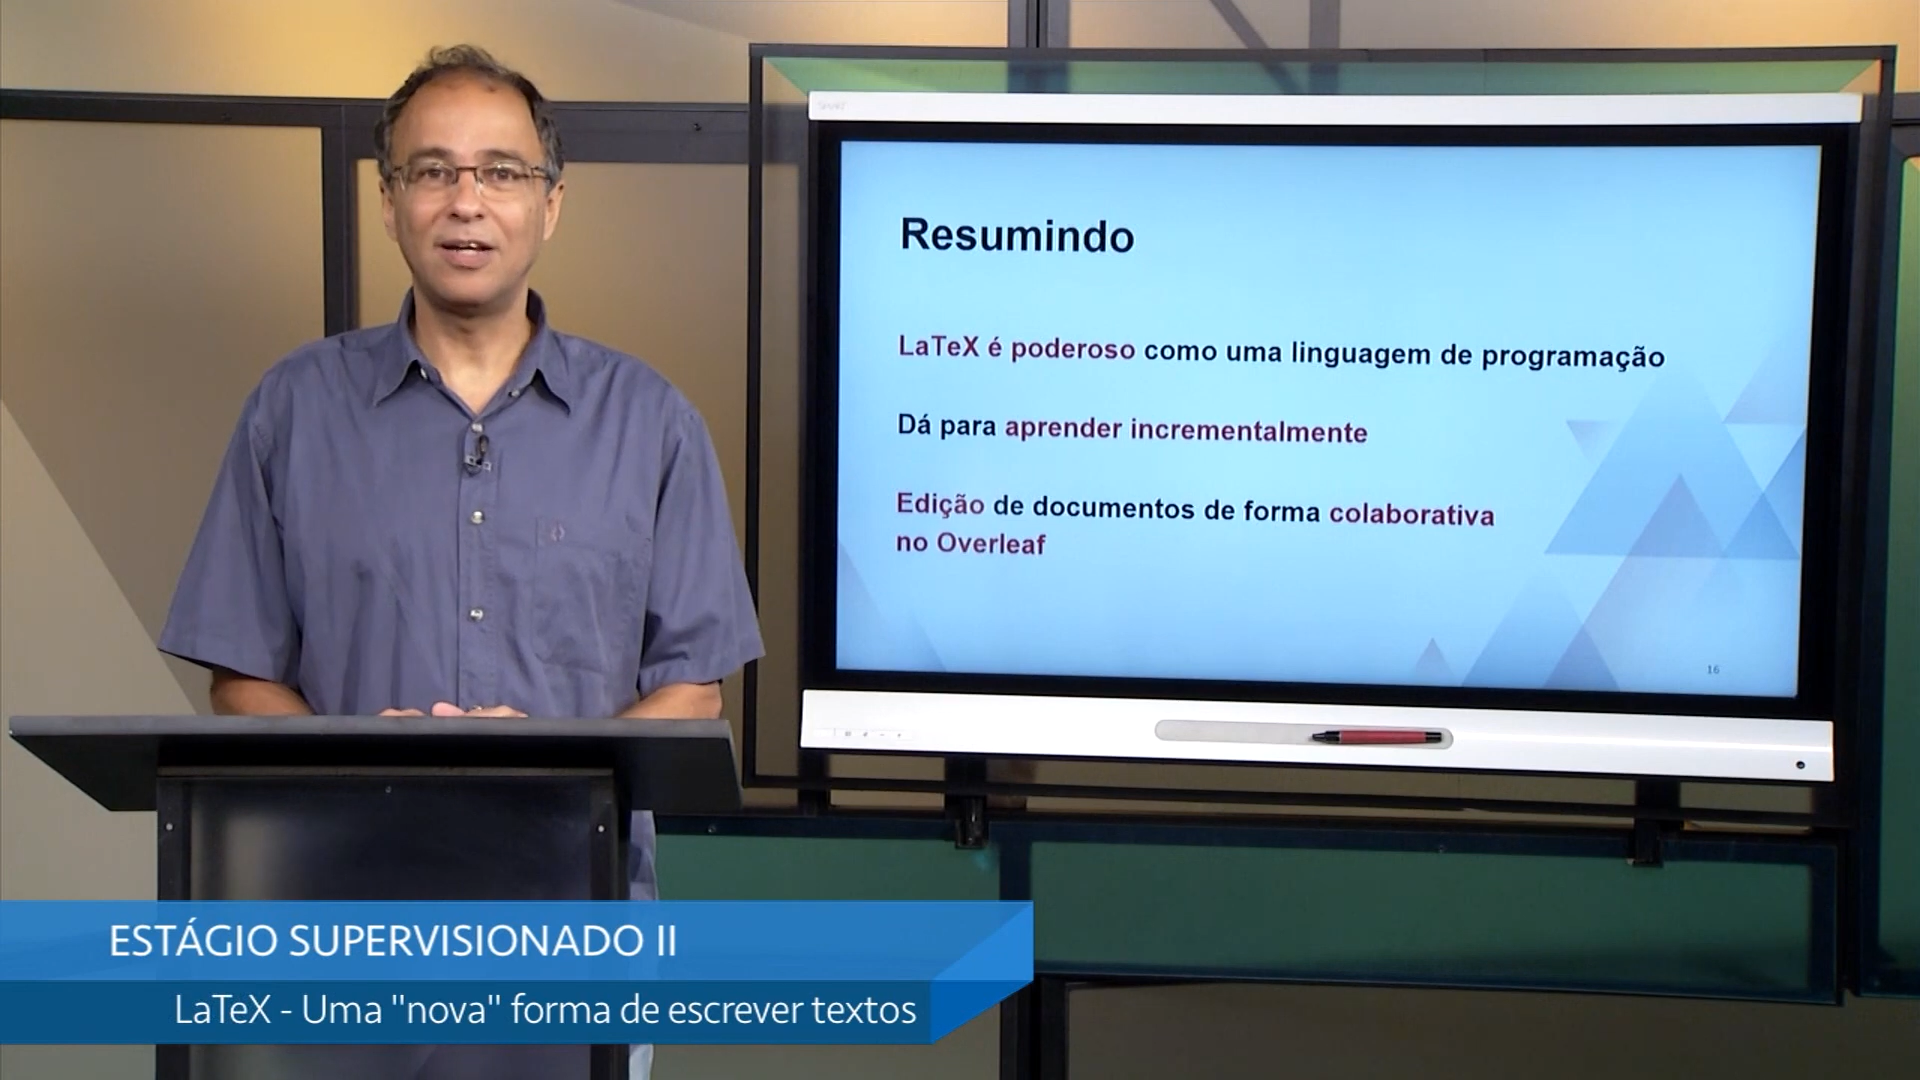
\includegraphics[width=0.5\textwidth]{overleaf.png} % Substitua com o caminho para sua imagem
      \captionsetup{labelformat=simple, labelsep=period}
      \caption{UNIVESP Estágio Supervisonado II - Eng. Comp.}
    \end{figure}
    
  \begin{center}
    Use LaTeX/Overleaf para fazer o texto!\\
  \end{center}
  \href{https://integra.univesp.br/courses/1898}{https://integra.univesp.br/courses/1898}\\
  
  \href{https://www.youtube.com/watch?v=AYc5mG9cOF4}{https://www.youtube.com/watch?v=AYc5mG9cOF4}\\
  
  \end{block}
\end{frame}

\begin{frame}
  \frametitle{Outras Dicas - "Mão na Roda"}
  \begin{block}{}
    \begin{figure}
      \centering
      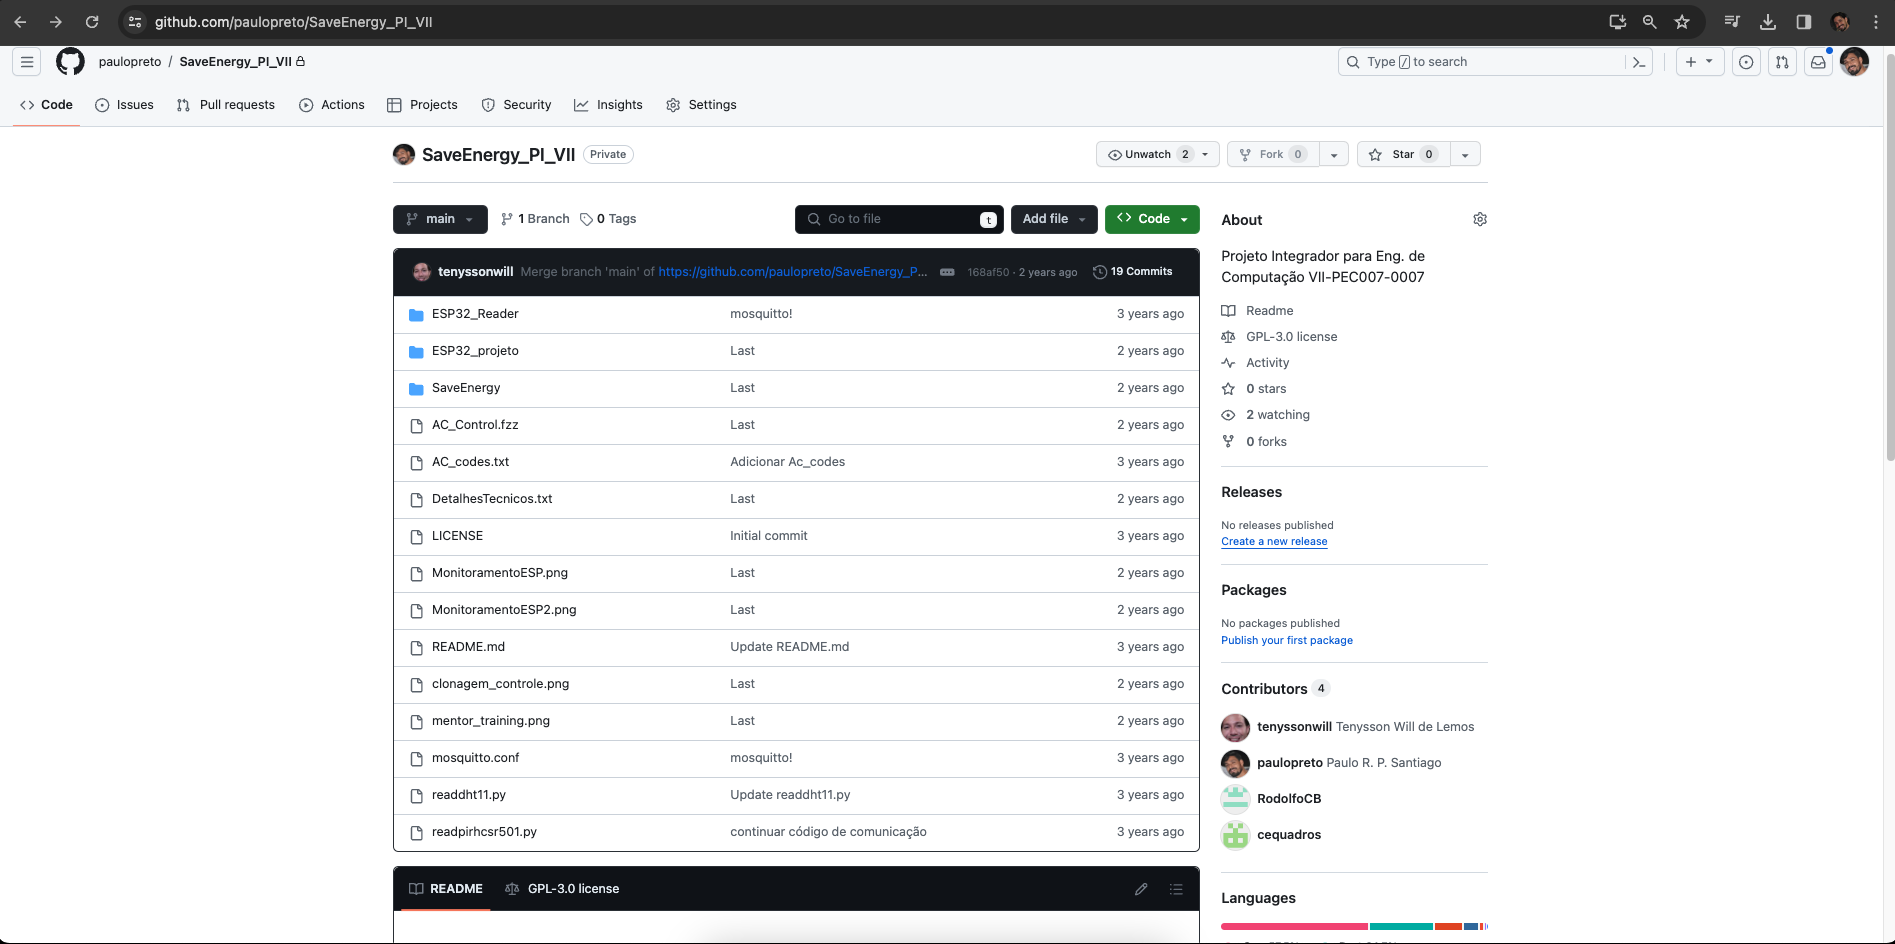
\includegraphics[width=0.9\textwidth]{github_pi.png} % Substitua com o caminho para sua imagem
      \captionsetup{labelformat=simple, labelsep=period}
      \caption{GitHub do PI.}
    \end{figure}
  \end{block}
\end{frame}

\begin{frame}
  \frametitle{Outras Dicas - "Mão na Roda"}
  \begin{block}{}
    \begin{figure}
      \centering
      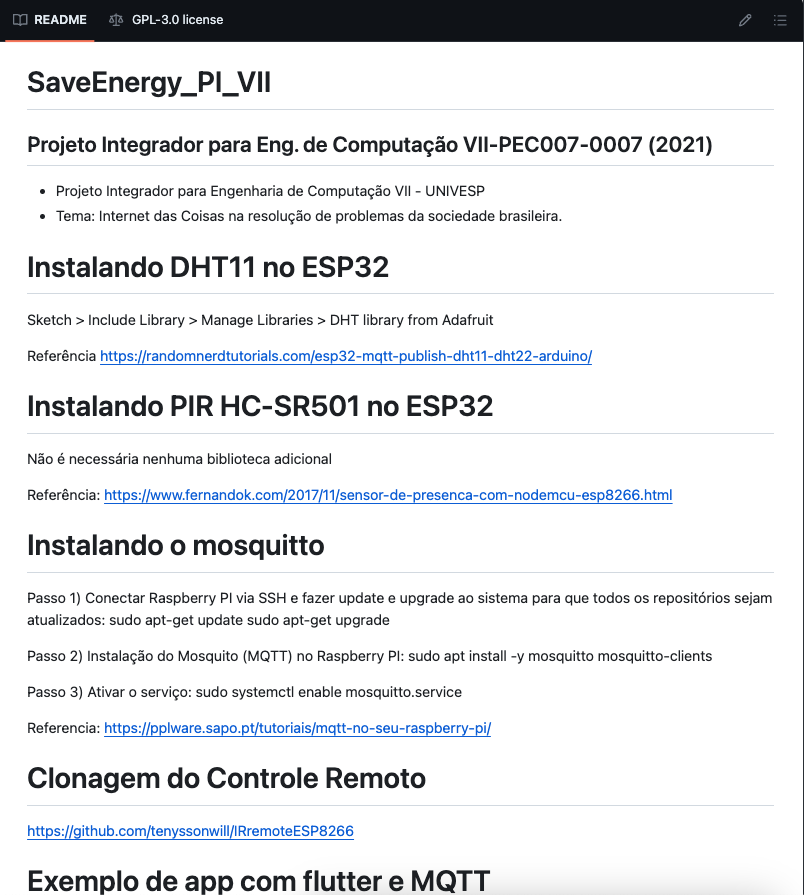
\includegraphics[width=0.5\textwidth]{readme_md.png} % Substitua com o caminho para sua imagem
      \captionsetup{labelformat=simple, labelsep=period}
      \caption{README.md em Markdown.}
    \end{figure}
  \end{block}
\end{frame}


\begin{frame}
  \frametitle{Outras Dicas - "Mão na Roda"}
  \begin{minipage}{0.48\textwidth}
    \centering
    \begin{figure}
      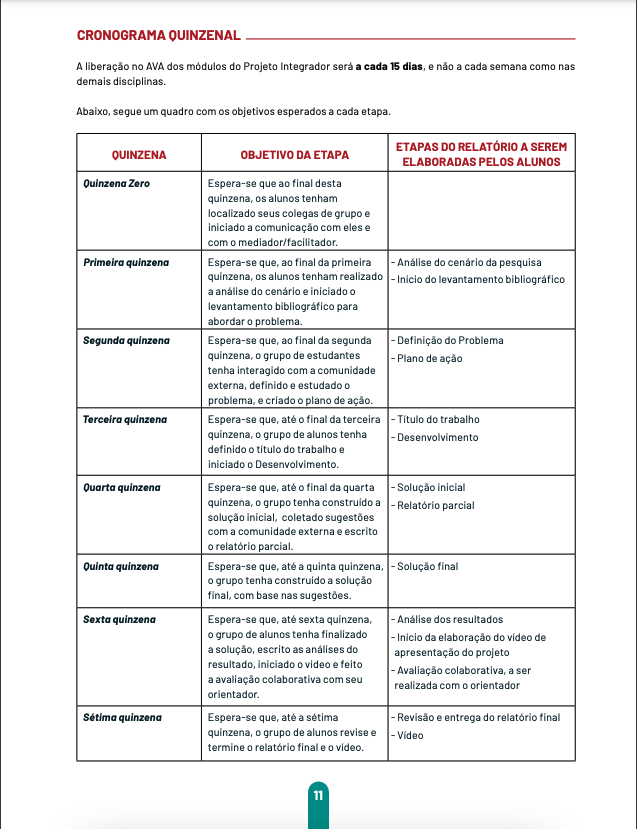
\includegraphics[width=\textwidth]{cronograma.png}
      \captionsetup{labelformat=simple, labelsep=period}
      \caption{Cronograma.}
    \end{figure}
  \end{minipage}
  \hfill
  \begin{minipage}{0.48\textwidth}
    \centering
    \begin{figure}
      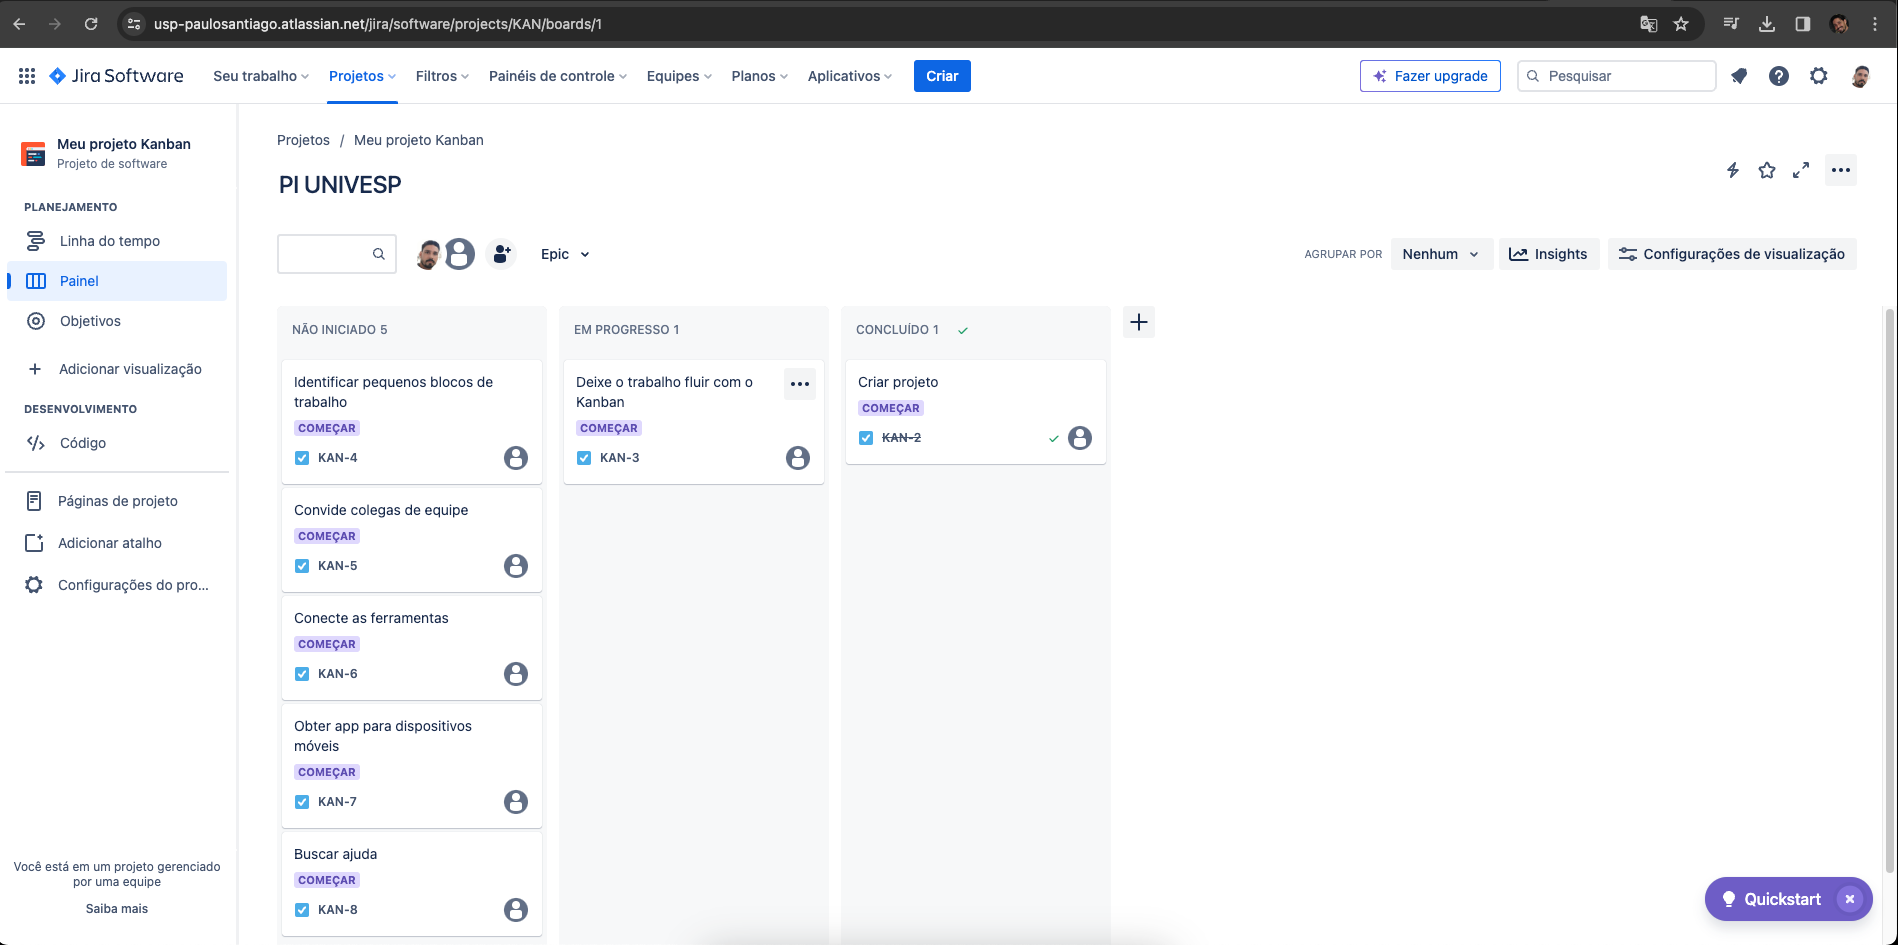
\includegraphics[width=\textwidth]{jira.png}
      \captionsetup{labelformat=simple, labelsep=period}
      \caption{Faça no Jira.}
    \end{figure}
  \end{minipage}
\end{frame}


\begin{frame}
  \frametitle{Obrigado!}
  \centering

  % Logos da USP e UNIVESP lado a lado
  
\includegraphics[height=3em]{usp-logo-png-1.png}\hspace{2mm}
  
\includegraphics[height=2.5em]{univesp.png}\\
  Paulo Roberto Pereira Santiago\\
  \href{mailto:paulosantiago@usp.br}{\texttt{paulosantiago@usp.br}}

  
  \vspace{5mm} % Espaçamento vertical
  % Links de contato com texto reduzido
  \begin{tiny}
  \href{https://github.com/paulopreto}{
\includegraphics[height=3em]{github-logo.png}\\
  https://github.com/paulopreto}
  
  \href{www.linkedin.com/in/paulo-roberto-pereira-santiago-132619112/}{
\includegraphics[height=3em]{LinkedIn_logo.png}\\ www.linkedin.com/in/paulo-roberto-pereira-santiago-132619112/}\\
  \href{http://www.eeferp.usp.br/?q=pt-br/funcionario/paulo-roberto-pereira-santiago}{
\includegraphics[height=3em]{eeferp.jpeg}\\ http://www.eeferp.usp.br/?q=pt-br/funcionario/paulo-roberto-pereira-santiago}\\
  \href{https://ibm.fmrp.usp.br/docentes-conexao-informatica-biomedica}{
\includegraphics[height=3em]{Infor-IBm-logo.png}\\ https://ibm.fmrp.usp.br/docentes-conexao-informatica-biomedica}
  \end{tiny}
\end{frame}




\end{document}
